% Chapter 5

\chapter{Experimente} % Main chapter title

\label{Chapter5} % For referencing the chapter elsewhere, use \ref{Chapter1}

%----------------------------------------------------------------------------------------

\begin{itquote}
Q: Why did the multithreaded chicken cross the road?\\
A: to To other side . get the
\flushright
\textsc{Jason Whittington}
\end{itquote}

Dieses Kapitel ist den drei in dieser Arbeit ausgeführten Experimenten gewidmet. Diese entsprechen
\begin{itemize}
  \item[$\mathcal{A}$:] Reproduktion des Ansatzes von (\cite{bordes2013translating}) mit einem kleineren Datenset
  \item[$\mathcal{B}$:] Training von Relationsrepräsentationen ähnlich (\cite{bordes2013translating}) mit Wortkontextvektoren
  \item[$\mathcal{C}$:] Identifikation von Wortpaaren gleicher Relation durch Clustering
\end{itemize}
In jedem Unterkapitel wird das jeweilige Prozedere beschrieben sowie die gewonnen Ergebnisse evaluiert. Zuletzt folgt
jedes Mal ein Zwischenfazit. Ein Resümee für alle Versuche wird danach in Kapitel \ref{Chapter6} gezogen.

\section{Experiment $\mathcal{A}$: TransE für deutsche Wissensdaten}\label{sec:exp-a}

In diesem Unterkapitel soll der Ansatz von (\cite{bordes2013translating}) für deutsche Daten nachvollzogen werden.
Dabei wird erst erklärt, wie die Daten erstellt wurden. Danach wird die Idee zum Training der Daten weiter ausgeführt und
auf die neuen Datensätze angewendet, bevor schlussendlich eine Evaluation und eine Gegenüberstellung zu den Originalergebnissen
erfolgt.

\subsection{Datenerzeugung}

In (\cite{bordes2013translating}) werden mehrere Relationsdatensets erstellt, darunter eines namens \textsc{FB15k}. Dieses
besteht aus Relationstripeln der Form $(h, l, t)$\footnote{= $(head,\ link,\ tail)$}, wobei
$h$ und $t$ Entitäten und $l$ die verbindende Relation bezeichnen. Diese stammen aus \emph{Freebase}, einer
von einer Onlinegemeinschaft gepflegten Datenbank, in der mehr als 23 Millionen Entitäten durch Relationen miteinander verknüpft sind.
Mittlerweile ist die Seite offline; das Projekt wurde sukzessive in \emph{Wikidata}\footnote{Siehe \url{https://www.wikidata.org/wiki/Wikidata:Main_Page (zuletzt abgerufen am 20.05.16)}} integriert. Auch die
\emph{Freebase API}, die als Programmierschnittstelle zum Abfragen von Informationen dient, wird langsam abgeschaltet
\footnote{Siehe \url{https://en.wikipedia.org/wiki/Freebase (zuletzt abgerufen am (20.05.16))}}.\\

Die \textsc{FB15k}-Daten enthalten 592.213 Tripel mit 14.951 einzigartigen Entitäten und 1.345 einzigartigen Relationen.
In \emph{Freebase} sind Entitäten generell sprachlich unabhängig gehalten. So wird die Entität mit dem Kürzel \verb|/m/02vk52|
im Englischen mit dem Begriff \emph{World Bank} und im Deutschen mit \emph{Weltbank} bezeichnet. Somit ist auch
\textsc{FB15k} zumindest theoretisch mehrsprachig, da es nur die \textsc{Freebase}-Kürzel enthält.
Jedoch sind die Entitäten darin oft hauptsächlich im englischen bzw. amerikanischen Sprachraum relevante
Entitäten, die im deutschen Raum teils nicht sehr bekannt sind. Diese 1:1 ins Deutsche zu übernehmen gestaltet sich schwierig,
da nicht jedes Kürzel in \emph{Freebase} mit einer deutschen Bezeichnung aufgeführt ist. Das könnte jeweils drei Gründe haben:

\begin{enumerate}
  \item Es gibt keine deutsche Übersetzung
  \item Die Entität ist für den deutschen Sprachraum nicht relevant genug
  \item Bisher hat einfach kein Nutzer einen deutschen Begriff hinzugefügt
\end{enumerate}

Die Plausibilität dieser Gründe ist diskutabel: Nicht alle Begriffe brauchen eine Übersetzung, so sind beispielsweise
Personennamen i.d.R. durch alle Sprachen hinweg gleich. Schwieriger wird es bei Ortsnamen oder Namen von Organisationen:
Intuitiv drängt sich der Anschein auf, dass populäre Bezeichnungen eher übersetzt werden als unpopulärere
(\emph{United States of America} $\rightarrow$ \emph{Vereinigte Staaten von Amerika} \textbf{aber} \emph{University of Denver}
$\rightarrow$ \emph{University of Denver}).\\
Im Falle der Relevanz ist davon auszugehen, dass diese mit der Anzahl der Nutzer einher geht: Bei einer großen
Nutzerbasis ist davon auszugehen, dass diese primär Einträge von Entitäten bearbeiten, die im Kontext der Geschichte,
des Tagesgeschehens o. Ä. relevant sind. Gegeben genug Zeit und aktive Nutzer ist also anzunehmen, dass eine immer
größer werdende Prozentzahl von relevanten Entitäten an das Deutsche angepasst wird. Bedenkt man die Laufzeit von Freebase
seit 2007 (also zum Zeitpunkt des Schreibens dieser Arbeit rund 9 Jahre), so nehmen wir an, dass dieses Bedenken zwar nicht
ganz aus der Welt zu räumen, aber zumindest zu vernachlässigen ist.\\

Basierend auf dieser Argumentation werden korrespondierende ``deutsche'' Daten folgendermaßen erzeugt:
Es wird bei allen Relationstripeln eine Prüfung durchgeführt, ob beide Entitäten $h$ und $t$ eine deutsche Bezeichnung
besitzen. Falls nicht, wird dieses Tripel ausgelassen. Danach wird ggf. noch die inverse Relation ergänzt (diese wird
später beim Training benötigt), z.B. bei \emph{/location/location/contains} und \emph{/location/location/containedby}.

\begin{table}[h]
  \centering
  \def\arraystretch{1.5}
  \begin{tabular}{@{}lrrr@{}}
    \toprule
    \textsc{Datenset} & \textsc{\#Tripel} & \textsc{\#Entitäten} & \textsc{\#Relationen} \\
    \toprule
    FB15k & 592.213 & 14.951 & 1.345 \\
    GER14k & 459.724 & 14.334 & 1.236 \\
    \bottomrule
  \end{tabular}
  \caption[Daten über die Relationsdatensets FB15k und GER14k]{Daten über die Relationsdatensets FB15k und GER19k.
  Aufgelistet ist die Anzahl der Tripel (Datensätze) und der einzigarten Entitäten und Relationen (\emph{Entitäts-} bzw.
  \emph{Relationstypen}).\label{fig:fb15kger14k}}
\end{table}

Somit gilt für die Menge englischer Relationstripel $S_{EN}$ und die Menge deutscher Tripel $S_{DE}$, dass letztere
eine echte Teilmenge ist: $S_{EN} \supsetneq S_{DE}$ \footnote{$\forall e \in S_{DE}: e \in S_{EN} \wedge S_{DE} \neq S_{EN}$}.
Verschiedene Informationen über die beiden Datensets sind in Abbildung \ref{fig:fb15kger14k} aufgelistet.

\subsection{Training}

Gegeben ist eine Menge von Relationstripeln $S$ der Form $(h, l, t) \in S$. Zusätzlich gibt es noch eine Entitätsmenge
$E$ sodass $h, t \in E$ und eine Menge von Relationen $L$ mit $l \in L$. Den Entitäten und Relationen werden zusätzlich
noch Vektoren zugewiesen, sodass $h, l, t \in \mathbb{R}^k$ gilt. Idealerweise gelten nach dem Training für ein gültiges Tripel $(h, l, t)$
dann $h + l \approx t$. Hinzu wird noch eine Menge aus korrumpierten bzw. ``falschen'' Tripeln $S'$ erstellt, indem
für jedes Tripel in $S$ entweder $h$ oder $t$ durch eine andere, zufällig gewählte Entität ersetzt wird:
\begin{equation}
  S' = \{(h', l, t) | h' \in E\} \cup \{(h, l, t') | t' \in E\}
\end{equation}

Diese Methode wird von (\cite{bordes2013translating}) rauschkontrastierendes Lernen (\emph{Noise-contrastive learning})
genannt.

Um die für das Training benötigte Verlustfunktion zu definieren, wird das Unähnlichkeitsmaß $d_p$ für ein Tripel bestimmt, welcher
entweder aus der $L_1$- oder der $L_2$-Norm abgeleitet wird, also:
\begin{equation}
    d_1(h + l, t) = \sum_{i=1}^k \| h_i + l_i - t_i \|
\end{equation}
\begin{equation}
    d_2(h + l, t) = \sqrt{\sum_{i=1}^k \| h_i + l_i - t_i \|^2}
\end{equation}

Zuletzt werden noch Tripel $s$ aus $S$ und zufällige Tripel $s'=(h', l, t')$ aus $S'$ in Pärchen in einem neuen Datenset $S^*$ gruppiert:
\begin{equation}
  S^* = \{(s, sample(S'))| s \in S\}
\end{equation}

Nun kann die Verlustfunktion $\mathcal{L}$ erstellt werden:
\begin{equation}\label{form:lossf}
  \mathcal{L} = \sum_{((h,l,t), (h', l, t')) \in S^*} max(0, \gamma + d_p(h + l, t) - d_p(h' + l, t'))
\end{equation}

Der Parameter $\gamma$ bezeichnet hier einen Hyperparameter, der dem System einen gewissen Spielraum lässt. Indem versucht
wird, den durch diese Funktion errechneten Verlust zu minimieren, wird beim Training sichergestellt, dass die Vektorrepräsentationen
von korrekten Tripeln die Gleichung $h + l \approx t$ bestmöglichst erfüllen und für korrumpierte Tripel möglichst weit
verfehlen.\\

Vor dem Training werden die Repräsentationen der Entitäten und Relationen mit einer uniformen Verteilung im Intervall
$[-\frac{6}{\sqrt{k}}, \frac{6}{\sqrt{k}}]$ initialisiert und im Falle von $l \in L$ zusätzlich normiert. Während jedem
Trainingsschritt wird für die aktuelle Repräsentation der Verlust berechnet und deren Werte mithilfe des
\emph{minibatch stochastic gradient descent}-Algorithmus angepasst. Die Minibatch enthält dabei ebenso viele gültige wie korrumpierte Tripel.
Das Training wird solange ausgeführt, bis die Fehlerrate auf dem Validationsset konvergiert\footnote{Konvergenz auf dem
Trainingsset könnte ein Zeichen für Overfitting sein.}.\\

Für das Reproduzieren der Ergebnisse wurde den Empfehlungen von (\cite{bordes2013translating}) gefolgt: So wird das Training
nach maximal 1000 Epochen beendet, außerdem gilt $k = 50$, $\gamma = 1$, $\lambda = 0,01$ und $d_1$ als Unähnlichkeitsmaß.

\subsection{Evaluation}\label{sec:transe-eval}

Um die erstellten Daten zu evaluieren, wurden bei den Relationen im Testset jeweils die Kopf- und Fußentitäten entfernt.
Danach wurden alle bekannten Entitäten aus $E$ eingesetzt und mithilfe des Unähnlichkeitsmaßes ansteigend sortiert. Der Rang
der korrekten (ursprünglich entfernten) Entität wurde dann gespeichert. Dieses Verfahren wurde zuerst von (\cite{bordes2011learning})
vorgeschlagen.\\

Daraus lassen sich zwei Evaluationsmaße ableiten: Den gemittelten Rang der korrekten Entität sowie den Anteil
der Evaluationsläufe, bei denen sich die richtige Entität innerhalb der Top 10 befand (Hits@10). Zusätzlich wurde noch
zwischen roh und gefiltert unterschieden: Bei letzterem werden mögliche Tripel ignoriert, die in dieser Form zufällig schon in
den Trainingsdaten vorkamen und so auf ``unfaire'' Art und Weise vor allen anderen Tripeln bevorzugt werden.
Als Baseline wurde eine Methode namens \emph{Unstructured} aus (\cite{bordes2013translating}) verwendet, bei denen
die Relationsvektoren einfach Nullvektoren entsprechen.
Die Ergebnisse für die auf FB15k und GER14k trainierten Daten sind in Abbildung \ref{fig:results1} festgehalten.

\begin{table}[h]
  \centering
  \def\arraystretch{1.5}
  \begin{tabular}{@{}lrrrr@{}}
    \toprule
     & \multicolumn{2}{c}{\textsc{\O\ Rang}} & \multicolumn{2}{c}{\textsc{Hits@10}} \\ \cmidrule(l{2pt}r{2pt}){2-3} \cmidrule(l{2pt}r{2pt}){4-5}
     \textsc{Datenset} & \emph{Roh} & \emph{Gefiltert} & \emph{Roh} & \emph{Gefiltert} \\
     \toprule
     \textsc{Unstr.} & 1123,46 & 1123,46 & 5,75 & 5,75 \\
     \textsc{FB15k} & 575,54 & \textbf{197,02} & \textbf{34,8} & \textbf{48,79} \\
     \textsc{GER14k} & \textbf{234,73} & 222,05 & 34,07 & 41,83 \\
     \bottomrule
  \end{tabular}
  \caption[Resultate für TransE mit \textsc{FB15k} und \textsc{GER14k}]{Resultate für TransE, trainiert auf dem
  \textsc{FB15k}- und dem \textsc{GER14k}-Datenset. Evaluiert gegen Unstructured (\textsc{Unstr.}), wobei einfach
  Nullvektoren als Relationsvektoren fungieren.\label{fig:results1}}
\end{table}

An den Ergebnissen ist zuerst zu erkennen, dass sie von den Ergebnissen in (\cite{bordes2013translating}) für FB15k etwas abweichen.
Dies könnte daran liegen, dass bei der Beschreibung des Trainingsverfahren angegeben wurde, dass das Prozedere
nicht unbedingt 1000 Epochen lang ausgeführt wurde. In dem Code, der von den Autoren online zur Verfügung gestellt und
zum Training verwendet wurde\footnote{\url{https://github.com/glorotxa/SME}}, wurde dazu leider keine entsprechende Option gefunden, weshalb vermutlich davon auszugehen
ist, dass dies manuell ausgeführt oder nicht im Code festgehalten wurde.
Daraus ist zu schließen, dass die hier aufgeführten Ergebnisse schlechter sind als die,
die im Paper angegeben wurden, weil die Vektorrepräsentationen zu sehr auf die Trainingsdaten angepasst wurden und dann schlecht
auf den Testdaten generalisieren. Da die Daten aus \textsc{GER14k} eine Untermenge von \textsc{FB15k} sind, sind deren Ergebnisse
i.d.R. gleichwertig oder schlechter. Die Frage, warum der rohe gemittelte Rang bei \textsc{GER14k} signifikant besser ist als
bei FB15k, könnte dahingehend beantwortet werden, dass auch hier eine übermäßige Anpassung auf die Trainingsdaten stattfand und
zuviele Trainingstripel vor der eigentlich richtigen Lösung rangieren. Deshalb ist der Wert für die gefilterten Tripel umso
besser.

\subsection{Zwischenfazit}

In diesem Kapitel wurde ein Verfahren vorgestellt, das es erlaubt, Vektorrepräsentationen zu trainieren, die Entitäten und Relationen
aus Wissensdatenbanken modellieren und zur Relationsvorhersage genutzt werden können. Dabei bestehen die Daten aus Relationstripeln,
also 3-Tupeln mit einer Kopf- und einer Fußentität und einer dazugehörigen semantischen Relation. Es werden außerdem noch
Negativbeispiele erzeugt, indem eine der beiden Entitäten durch eine andere in den Trainingsdaten vorkommende Entität zufällig ausgetauscht wird.
Der Trainingsvorgang wird hierbei mithilfe eines auf Vektorarithmetik basierenden Unähnlichkeitsmaß betrieben, mit der
die ``Stimmigkeit'' korrekter Tripel versucht wird zu maximieren. Das Gegenteil gilt für korrumpierte Tripel.\\
Es wurde gezeigt, dass sich die in (\cite{bordes2011learning}) präsentierten Ergebnisse im Rahmen der gegebenen Möglichkeiten
annähernd replizieren lassen. Darüber hinaus wurde die Methodik auch auf eine Menge deutscher Daten angewendet, die eine
echte Teilmenge der englischen Daten darstellt. Für diese konnten ähnlich gute Ergebnisse erziehlt werden, wobei die qua
definitionem kleinere Menge an Übungsbeispielen dem Unterschied in der Performanz begründet.\\

Bei dieser Vorgehensweise wurden die Vektorrepräsentationen für Entitäten und Relationen gemeinsam trainiert. In den folgenden
Experimenten soll ein Versuch unternommen werden, mithilfe von distributioneller Semantik erstellte Wortvektorrepräsentationen
für die Entitäten zu nutzen und darauf aufbauend für ähnliche Zwecke wie in diesem Kapitel zu nutzen.\\

\section{Experiment $\mathcal{B}$: Relationsvorhersage mit Wortkontextvektoren}\label{sec:exp-b}

In diesem Unterkapitel soll versucht werden, die Methodik des rauschkonstrastierenden Lernen aus dem vorherigen Experiment
auf die Wortkontextvektoren (vgl. Kapitel \ref{Chapter4}) anzuwenden und nur die Relationsvektoren zu lernen. Zu diesem Zweck
wird eine Untermenge von \textsc{FB15k} gebildet, die Tripel enthält, deren Kopf- und Fußentität jeweils als Wortvektorrepräsentation vorliegen.
Schlußendlich werden die Ergebnisse evaluiert und diskutiert.

\subsection{Datenerzeugung}

Zu Trainingszwecken wird eine Untermenge aus \textsc{FB15k} bzw. \textsc{GER14k} gebildet. Da
die Vektorrepräsentationen für die Entitäten nicht von Grund auf erstellt sorden mit
\verb|word2vec| trainierte Vektoren verwendert werden, können nur solche Worte in dem
neuen Trainingsset vorhanden sein, zu denen ebensolche Wortvektoren auch vorliegen.
Dies ist leider nur für einen substantiell geringeren Teil der Fall, wie in Abbildung \ref{fig:we4k} zu
erkennen ist.

\begin{table}[h]
  \centering
  \begin{changemargin}{0cm}{0cm}
  \resizebox{\textwidth}{!}) & 14.334 & (\textcolor{BrickRed}{$\downarrow$-4,12 \%}) & 1.236 & (\textcolor{BrickRed}{$\downarrow$-8,1 \%}) \\
    WE4k & 50.518 & (\textcolor{BrickRed}{$\downarrow$-91,47 \%}) & 3.623 & (\textcolor{BrickRed}{$\downarrow$-74,72 \%}) & 749 & (\textcolor{BrickRed}{$\downarrow$-39,40 \%}) \\
    \bottomrule[1.25pt]
  \end{tabular}%
  }
\end{changemargin}
  \caption[Daten des neuen Relationsdatensets im Vergleich zu \textsc{FB15k} und \textsc{GER14k}]{Daten des neuen Sets \textsc{WE4k} im Vergleich mit
  \textsc{FB15k} und \textsc{GER14k}. Aufgelistet ist die Anzahl der Tripel (Datensätze), Entitäts- und Relationstypen und die Veränderung
  der Anzahlen in Prozent im Vergleich zu \textsc{FB15k} in Klammern.\label{fig:we4k}}
\end{table}

Dies ist dadurch zu erklären, dass in der Quelle der Originaldaten, nämlich \emph{Freebase},
sehr viele sehr seltene Entitäten vertreten sind. Die vielen Freiwilligen, die über die
Jahre dazu beigetragen haben, die Wissensdatenbank weiter zu vervollständigen, haben dabei auch
viele unbekanntere Filme, Personen etc. hinzugefügt, die in einem Korpus eher selten zu finden sind, sei er auch
so groß wie \textsc{Decow}.\\

Da die resultierende Menge an Tripeln gerundet ungefähr viertausend einzigartige Entitäten enthält, die auch als
Wortkontextvektoren vorliegen, wird dieses Datenset im Folgenden \textsc{WE4k} genannt.

\subsection{Training}

Das Training der Relationsvektoren findet in einer zu der in Kapitel \ref{Chapter6} beschrieben Methode sehr
ähnlichen Art und Weise statt: Es wird zuerst eine Menge korrumpierter Tripel erstellt, bei denen entweder
die Kopf- oder Fußentität ersetzt wurde.
Mithilfe der ursprünglichen Tripel wird eine Menge aus Tripelpaaren erstellt, von denen der korrumpierte Teil jeweils
zufällig aus $S'$ ausgewählt wird. Auch die Verlustfunktion gestaltet sich prinzipiell gleich (siehe Formel \ref{form:lossf}).\\

Die wenigen Unterschiede bestehen darin, dass diesmal nur die Repräsentationen der Relationen trainiert werden,
da die der Enitäten schon vorliegen, sowie im Trainingsschritt selbst: So wird wird wegen der geringeren Menge an
Daten darauf verzichtet, für jede Trainingsanzahl eine feste Anzahl von Tripelpaaren zufällig auszuwählen.
Stattdessen richtet sich die Größe von $S_{batch}$ nach folgender Formel\footnote{Die Addtion von 1 dient dazu, bei weniger
als 10 Tripeln für eine Relation wenigstens mit einem Tripel zu trainieren. Der Rest entspricht einer Heuristik. Es wurden
verschiedene Größen für den Minibatch ausprobiert, die jedoch keinen signifikaten Einfluss auf die Ergebnisse hatten.}:

\begin{equation}
  S_{batch} \leftarrow sample(S^*, \floor*{\frac{|S^*|}{10}}+1)
\end{equation}

\subsection{Evaluation}

Die Evaluation fand auf diesselbe Art und Weise wie im Abschnitt \ref{sec:transe-eval} statt. So wurde wieder untersucht,
inwiefern die Relationsvektoren und die Vektorrepräsentationen der Entitäten dazu genutzt werden können, ein Relationstripel
durch ``Raten'' zu vervollständigen und gemessen, welcher Rang der richtigen Antwort zugewiesen wurde und in wieivel Prozent
diese unter den besten Zehn anzutreffen war. Als Baseline fungierte wieder die \emph{Unstructured}-Methode, wobei die Relationsvektoren
Nullvektoren entsprechen.

\begin{table}[h]
  \centering
  \begin{tabular}{lrr}
    \toprule[1.5pt]
    \textsc{Datenset} & \textsc{\O\ Rang} & \textsc{Hits@10} \\
     \toprule
     \textsc{Unstr.} & 1123,46 & 5,75 \\
     \textsc{WE4k} & 1122,03 & 5,67 \\
     \textsc{FB15k} & \textbf{197,02} & \textbf{48,79} \\
     \textsc{GER14k} & 222,05 & 41,83 \\
    \bottomrule[1.25pt]
  \end{tabular}
  \caption[Resultate auf mit Wordvektoren auf \textsc{WE3k}]{Evaluationsergebnisse von \textsc{WE4k} gegenüber denen
  von \textsc{FB15k} und \textsc{GER14k} sowie der Unstructured-Baseline.\label{fig:eval-we4k}}
\end{table}

Im Blick auf Abbildung \ref{fig:eval-we4k} zeigt ein ernüchterndes Fazit auf. So schnitt die Variante
mit Wortvektoren aus \verb|word2vec| und seperat trainierten Relationsrepräsentationen ($\rightarrow$ \textsc{WE4k}) im Bezug auf
den gemittelten Rang mehr als fünf Mal so schlecht und im Bezug auf die \textsc{Hits@10} mehr als acht Mal so schlecht ab (sic!),
sogar ein wenig schlechter als die \emph{Unstructured}-Baseline.
Die möglichen Gründe für das weite Verfehlen guter Ergebnisse werden nun in Kapitel \ref{sec:we4k-zwifa} diskutiert.

\section{Zwischenfazit}\label{sec:we4k-zwifa}

Um die Diskrepanz zwischen den Ergebnissen mit gemeinsam trainierten Repräsentationen für Entitäten und Relationen im Vergleich
zu denen mit Wortkontext- als Entitätsvektoren zu erklären, sollte die Unterschiedlichkeit der Ansätze hervorgehoben
werden.\\

Im ersten Fall werden wie erwähnt alle eine Relation betreffende Repräsentationsvektoren gemeinsam trainiert; es ist
also davon auszugehen, dass diese bestmöglichst angepasst sind, um $\parallel h + r - t\parallel$ für alle $h, t$ zu minimieren.\\
Dies kann im zweiten Fall nicht unbedingt gewährleistet werden: Da $h$ und $t$ im Vornherein schon feststehen und nicht
an $r$ angepasst werden (sondern genau umgekehrt $r$ an $h$ und $t$ angepasst wird), kann der minimale Wert der Verlustfunktion
unter Umständen nur schwer erlangt werden.\\
Als weitere Begründungen sind anzuführen, dass
\begin{itemize}
 \item[a)] \textsc{WE4k} auf \textbf{deutlich} kleineren Datenmengen arbeitet (weshalb maschinelle
  Lernverfahren unter Umständen gar keine Lösung finden können, die gut auf ungesehene Beispiele generalisiert) und
  \item[b)] Wortkontextvektoren von sehr speziellen Entitäten enthält, die in \emph{Freebase} als Knoten existieren,
  unter Umständen aber sehr selten im Korpus auftauchen
\end{itemize}
Da die Beschaffenheit der korpusbasierten Repräsentationen vor allem von Kookkurrenzen mit anderen
Begriffen abhängt, bedeutet eine niedrige Termfrequenz vor allem weniger aussagekräftige Wortkontextvektoren, worunter die
Ergebnisse in der Konsequenz zu leiden haben.\\

Zuletzt sollte mit in Betracht gezogen werden, dass die trainierten Relationen sehr feingliedrig sind. Anderen Forschungsarbeiten,
 die mit grobaufgelösten Beziehungen wie ``Cause-Effect'' oder ``Entitiy-Origin''
(\cite{hendrickx2009semeval}) arbeiten, können dadurch auf größere Datenmengen zugreifen und bessere Ergebnisse auf
ungesehenen Beispielen erzielen.\\

Das nächste Experiment entfernt sich vom Training eigener Vektorrepräsentation und befasst sich mit der Frage, ob
$h + r \approx t$ genutzt werden könnte, neue Relationen auf Basis von Wortkontextvektoren auszumachen und bestehende um
 neue Wortpaare zu erweitern. Um diese Hypothese zu überprüfen, werden alle möglichen Vektorpaare durch ein
 Clusteringverfahren nach ihrem $r$ ($h + r \approx t \rightarrow r \approx t - h$) gruppiert.

\section{Experiment $\mathcal{C}$: Relationsvorhersage mit Wortvektorrepräsentationen}\label{sec:exp-c}

In diesem Unterkapitel wird ein unüberwachtes maschinelles Lernverfahren auf Wortkontextvektorpaare angewendet, um diese
nach ihrem Differenzvektor zu clustern. Diesbezüglich wird sich eines Algorithmus bedient, der aufgrund verschiedener
Faktoren immer weiter modifiziert wird.

\subsection{Idee}

Gegeben ist ein Vektorraum $V$ mit Wortkontextvektoren $\vec{u}, \vec{v} \in V = {R}^d$.
Gesucht ist eine Funktion $\phi$, die ein Vektorenpaar $(\vec{u}, \vec{v})$ in einen Relationsraum abbildet:
$\phi: \mathbb{R}^d \times \mathbb{R}^d \to \mathbb{R}^e$, wobei
nicht zwangsläufig $d = e$.\\
In ihrer einfachsten Form bildet sie einfach die Differenz $\vec{d}$ der beiden Vektoren ab:
\begin{equation}
  \phi(\vec{u}, \vec{v}) = \vec{v} - \vec{u} = \vec{d}
\end{equation}

\subsection{Algorithmus}

Der Grundalgorithmus (siehe Abbildung \ref{fig:algo1}) versucht nun, alle Kombinationen von Differenzen der
Wortkontextvektoren zu bilden. Die Berechnung dieser würde bei $n$ Vektoren in $O(n) = n * n = n^2$ resultieren.
Zwar ist $\phi(\vec{u}, \vec{v}) \neq \phi(\vec{v}, \vec{u})$, jedoch wäre die Berechnung beider Differenzvektoren redundant,
da sie lediglich Spiegelungen voneinander im Raum sind und so dieselbe Information enthalten. Die Berechnung
der Differenz in nur eine Richtung reduziert die Komplexität dadurch zu $O(n) = \frac{n * (n-1)}{2}$
\footnote{
Gegeben einer Menge relevanter Vektorpaarkombinationen $\mathcal{C}$ gilt also:
\[
  \forall (\vec{u}, \vec{v}) \in \mathcal{C}: (\vec{v}, \vec{u}) \notin \mathcal{C}
\]
}.

\begin{figure}[h]
  \centering
  \begin{algorithm}[H]
    \KwData{Menge von Vektorpaaren $\mathcal{C}$}
    \For{$(\vec{u}, \vec{v}) \in \mathcal{C}$}{
      $\vec{d} = \vec{v} - \vec{u}$;
    }
  \end{algorithm}
  \caption[Einfacher Projektionsalgorithmus]{Einfacher Projektionsalgorithmus.\label{fig:algo1}}
\end{figure}

Eine Modifikation des Algorithmus besteht darin, das Berechnen von $\vec{d}$ an eine Bedingung zu knüpfen, da selbst
mit der obigen Einschränkung die Ausgabe des Algorithmus gegeben einer Datenmenge immer noch sehr groß ist.\\

Gegeben sei eine Menge von Sätzen (ein Korpus) $\mathcal{K}$ mit $n$ Sätzen $s_0, \ldots, s_n$ sodass $\mathcal{K} = \{s_i\}_{i=1}^{n}$ mit
$m$ Wörtern $w_{ij}$ pro Satz $s_i = \{w_{ij}\}_{j=1}^m$. Eine Kookkurrenz von zwei Begriffen (\emph{types}) $t_1$ und $t_2$
besteht demnach, falls im Korpus mindestens ein Satz existiert, in dem beide vorkommen. Dazu können wir
eine Funktion $\Lambda(\cdot)$ definieren, die die Anzahl der Kookkurrenzen für alle Sätze $s_i$ und deren jeweiligen
Wörtern $w_{ij}$ bestimmt:
\begin{equation}\label{form:lambda-cooc}
  \Lambda(t_1, t_2) = |\{s_i | \exists w_{ij} = t_1 \land \exists w_{ij} = t_2 \land t_1\neq t_2\}_{i=1}^{n}|
\end{equation}
Eine mögliche Einschränkung besteht darin, in einem geänderten Algorithmus (siehe Abbildung \ref{fig:algo2}) das Berechnen von $\vec{d}$ nur
dann zu erlauben, wenn die Anzahl der Kookkurrenzen der zu den Vektoren $\vec{v}(t_1), \vec{v}(t_2)$ gehörenden Begriffe $t_1, t_2$
einen bestimmten Schwellenwert $\gamma$ überschreitet, also $\Lambda(t_1, t_2) \geq \gamma$.

\begin{figure}[h]
  \centering
  \begin{algorithm}[H]
    \KwData{Menge von Vektorpaaren $\mathcal{C}$}
    \For{$(\vec{v}(t_1), \vec{v}(t_2)) \in \mathcal{C}$}{
      \If{$\Lambda(t_1, t_2) > \gamma$}{
        $\vec{d} = \vec{v}(t_2) - \vec{v}(t_1)$;
      }
    }
  \end{algorithm}
  \caption[Modifizierter Projektionsalgorithmus]{Modifizierter Projektionsalgorithmus, bei dem die zu den Vektoren gehörigen
  Begriffe über $\gamma$ Mal im Korpus im gleichen Satz aufgetreten sein müssen, damit $\vec{d}$ errechnet wird.\label{fig:algo2}}
\end{figure}


\subsection{Parallelisierter Algorithmus}\label{sec:para-algo}

Doch selbst mit den erwähnten Einschränkungen skaliert dieser Algorithmus nur bedingt. Um dem entgegenzuwirken, soll nun
versucht werden, diesen mithilfe von \emph{Multithreading} zu parallelisieren. Bei dieser Technik beschäftigt ein Rechenprozess
mehrere Prozessstränge (\emph{Threads}), die miteinander kommunizieren und bei Bedarf synchronisiert werden können,
während sie Teile eines Problems gleichzeitig lösen.\\

Ein beliebtes Muster, das Verhältnis zwischen mehreren Threads zu definieren, besteht im \emph{Master-Slave}-Muster.
Dabei fungiert ein Subprozess als Aufseher, der seine Arbeiterprozesse überwacht, sie mit Daten versorgt und in manchen
Fällen untereinander koordiniert, während die anderen Prozesse Teilprobleme lösen und ggf. Rückmeldung an den Aufseherprozess
geben.\\

\begin{figure}[h]
  \centering
  \begin{algorithm}[H]
    \KwData{Menge von Vektorpaaren $\mathcal{C}$}
    \KwData{Menge von erledigten Vektorpaaren $\mathcal{C}'$ (Anfangs $\mathcal{C}' = \varnothing$)}
    \KwData{Menge von Threads $\mathcal{T}=\{th\}_i^n$}
    \BlankLine
    \textbf{Klasse} \textsc{MasterThread} \\
      data = ladeDaten();\\
      \For{$th \in \mathcal{T}$}{
        starteThread($th$, data);
      }
      \For{$th \in \mathcal{T}$}{
        beendeThread($th$);
      }

    \BlankLine
    \textbf{Klasse} \textsc{WorkerThread} \\
    \For{$(\vec{v}(t_1), \vec{v}(t_2)) \in \mathcal{C}$}{
      \If{$(\vec{v}(t_1), \vec{v}(t_2)) \notin \mathcal{C}'$}{
        \If{$\Lambda(t_1, t_2) > \gamma$}{
          $\vec{d} = \vec{v}(t_2) - \vec{v}(t_1)$;
        }
        $\mathcal{C}'$ = $\mathcal{C}' \cup (\vec{v}(t_1), \vec{v}(t_2))$;
      }
    }
  \end{algorithm}
  \caption[Parallelisierter Projektionsalgorithmus]{Parallelisierter Projektionsalgorithmus, bei dem die zu den Vektoren gehörigen
  Begriffe über $\gamma$ Mal im Korpus im gleichen Satz aufgetreten sein müssen, damit $\vec{d}$ errechnet wird. Ein Master-Thread
  verteilt zudem die Aufgaben an Worker-Threads, die diese Berechnungen übernehmen und erledigte Vektorpaare in einer Menge ablegen.
  \label{fig:algo3}}
\end{figure}

In diesem konkreten Fall ist der Master-Thread dafür verantwortlich, alle benötigten Daten in entsprechende Datenstrukturen
zu laden, sie den Worker-Threads bereitzustellen und letztere gemeinsam zu starten und zu beenden, sobald ein bestimmtes
Abschlusskriterium der Aufgabe erfüllt ist.
Zusätzlich wird eine Menge eingeführt, in der Paare von Vektoren hinzugefügt werden, sofern
ihr Differenzvektor von einem Thread ausgerechnet wurde (siehe Abbildung \ref{fig:algo3}). Damit nun keiner der Threads redundante Berechnungen durchführt, prüft er, ob sein
aktuelles Vektorpaar sich in dieser Menge befindet und schon abgehakt wurde\footnote{Damit dies möglichst schnell funktioniert,
wird das Vektorpaar durch eine Hashfunktion $h$ in einen Wert umgewandelt und in einem \emph{Hashset} gespeichert. $h(\cdot)$ wird so gewählt,
sodass $h(\vec{v}(t_1), \vec{v}(t_2)) = h(\vec{v}(t_2), \vec{v}(t_1))$.}.\\

Als Grundlage der Daten wurde das Datenset 01DERS5-5 gewählt, da es in den meisten der Evaluationsaufgaben
als bestes Abschnitt. Mit $\gamma = 1000$ resultierte das Prozedere in einer neuen Menge an Daten mit insgesamt
138.086 Differenzvektoren mit einer Größe von 117 Megabyte, ausgehend von einem Vektordatenset mit 6 Gigabyte und
ungefähr 6,6 Millionen Wortkontextvektoren.\\

\subsection{Evaluation}

Die Evaluation der im vorherigen Schritt gewonnen Daten findet folgendermaßen statt: Für jedes gewonnene Cluster $c$ wird für
jedes Paar von Vektoren die Zugehörigkeit der entsprechenden Wörter zu einer \textsc{Freebase}-Relation $r \in R$ geprüft.
Dem gesamten Cluster kann dann die Relation $r_c$ zugeordnet werden, die die meisten Treffer zu verzeichnet hat\footnote{Die Indikatorfuntion mit $\mathbbm{1}_{r_c}((w_1, w_2))$ liefert $1$, wenn
$(w_1, w_2) \in r$ gilt, ansonsten $0$.}:

\begin{equation}
    r_c = \underset{r \in R}{argmax}\ \sum_{(\vec{v}(w_1), \vec{v}(w_2)) \in c}  \mathbbm{1}_{r}((w_1, w_2))
\end{equation}

Die ``Reinheit'' $P$ eines Clusters kann dann errechnet werden, indem der Anteil der zur Relation des gesamten Clusters
zugehörigen Wortpaaren bestimmt wird:

\begin{equation}\label{form:purity}
    P(c) = \sum_{(\vec{v}(w_1), \vec{v}(w_2)) \in c} \frac{\mathbbm{1}_{r_c}((w_1, w_2))}{|c|}
\end{equation}

Diese Metrik bestraft es allerdings, wenn in einem Cluster neue Paare einer Relation vorkommen, die noch nicht in \textsc{Freebase}
vorhanden sind. Da es allerdings auch ein Teilziel dieses Ansatzes ist, ebensolche Paare neu aufzufinden, wird noch
eine modifizierte Version dieser Metrik behandelt: Es gilt dabei vor allem, unbekannte richtige Wortpaare von falschen
zu unterscheiden. Zu diesem Zweck wird die Annahme getroffen, dass alle Vektoren $\vec{v}(h)$ und $\vec{v}(t)$, die jeweils zu den Kopfentitäten $H_c$ und
den Fußentitäten $T_c$ gehören,
untereinander ähnlich sind:

\begin{equation}
H_c = \{\vec{v}(w_1)|(w_1, \cdot) \in r_c\}
\end{equation}

\begin{equation}
T_c = \{\vec{v}(w_2)|(\cdot, w_2) \in r_c\}
\end{equation}

In einem Cluster der Relation \emph{Hauptstadt von} würden sich so vermutlich die Vektoren aller Hauptstädte wie
\emph{Paris}, \emph{Berlin},$\ldots$ ebenso ähneln wie die der dazugehörigen
Länder \emph{Frankreich}, \emph{Deutschland},$\ldots$\\
So wird für jedes Cluster zunächst für ebendiese Entitäten ein Durchschnitt
errechnet, deren Zugehörigkeit zu $r_c$ festgestellt wurde:

\begin{equation}
  \overline{h} = \sum_{\vec{v}(w_1) \in H_c}\frac{\vec{v}(w_1)}{|H_c|}
\end{equation}

\begin{equation}
  \overline{t} = \sum_{\vec{v}(w_2) \in H_c}\frac{\vec{v}(w_2)}{|T_c|}
\end{equation}

Danach erweitern wir $r_c$ um die Wortpaare, deren Vektoren den durchschnittlichen Kopf- und Fußvektoren ähnlich genug sind.
Zu diesem Zweck wird ein Schwellenwert $\tau$ definiert, den ein potenziell zu $r_c$ zugehöriges Wortpaar im Bezug auf
Cosinusänlichkeit (siehe \ref{form:cossim}) nicht unterschreiten darf:

\begin{equation}
  r_c^+ = r_c\ \cup\ \{(w_1, w_2)| (\vec{v}(w_1), \vec{v}(w_2)) \in c\ \land\ cos(\vec{v}(w_1), \overline{h}) \geq \tau\ \land\ cos(\vec{v}(w_2), \overline{t}) \geq \tau\}
\end{equation}

Auf Basis der Gleichung \ref{form:purity} folgt für die modifizierte Reinheit eines Wortpaarclusters $P^+$:

\begin{equation}
  P^+(c) = \sum_{(\vec{v}(w_1), \vec{v}(w_2)) \in c} \frac{\mathbbm{1}_{r_c^+}((w_1, w_2))}{|c|}
\end{equation}

\subsection{Ergebnisse}

Vorgreifend soll angemerkt werden, dass es nicht möglich war, endgültige Ergebnisse mithilfe der vorher beschriebenen
Evaluationsmetrik $P^+(\cdot)$ zu erzeugen. Die genauen Gründe hierfür werden im nächsten Abschnitt \ref{sec:zwi-dis}
genauer beleuchtet. Dementsprechend sollen an dieser Stelle lediglich Zwischenergebnisse vorgestellt werden.\\

\begin{figure}[h]
  \centering
  \begin{multicols}{2}
    \textbf{Cluster A}\\
    \textsc{Oldenburg} - \textsc{Görlitz}\\
    \textsc{Tschechien} - \textsc{Karin}\\
    \textsc{Tschechien} - \textsc{Uwe}\\
    \textsc{Hockenheim} - \textsc{Offenburg}\\
    \textsc{Oldenburg} - \textsc{Offenburg}\\
    $\vdots$\\
    \columnbreak
    \textbf{Cluster B}\\
    \textsc{Pfeiffer} - \textsc{EU-Länder}\\
    \textsc{Franz} - \textsc{EU-Länder}\\
    \textsc{Uwe} - \textsc{EU-Länder}\\
    \textsc{Karin} - \textsc{EU-Länder}\\
    \textsc{Henning} - \textsc{EU-Länder}\\
    $\vdots$\\
  \end{multicols}
  \begin{multicols}{2}
    \textbf{Cluster C}\\
    \textsc{Nordhausen} - \textsc{Oberliga}\\
    \textsc{Bochum} - \textsc{Regionalliga}\\
    \textsc{Hameln} - \textsc{Regionalliga}\\
    \textsc{Chemnitzer} - \textsc{Regionalliga}\\
    \textsc{Chemnitzer} - \textsc{Bundesliga}\\
    $\vdots$\\
    \columnbreak
    \textbf{Cluster D}\\
    \textsc{Dieter} - \textsc{italienischen}\\
    \textsc{Pirna} - \textsc{italienischen}\\
    \textsc{Damon} - \textsc{italienischen}\\
    \textsc{Shanghai} - \textsc{italienischen}\\
    \textsc{Pankow} - \textsc{italienischen}\\
    $\vdots$\\
  \end{multicols}
  \caption[Auszug aus verschiedenen Wortpaarclustern]{Auszüge aus einigen Wortpaarclustern, die mit in dem Abschnitt
  \ref{sec:para-algo} vorgestellten Ansatz erzeugt wurden.\label{fig:clusters}}
\end{figure}

Wie Abbildung \ref{fig:clusters} zu entnehmen ist, in der einige Auszüge aus Clustern beispielhaft dargestellt sind,
fällt es schwer, die dort aufgeführten Wortpaare insgesamt einer Relation zuzuordnen. Im Gegenteil gelingt dies selbst für
einzelne Paare nicht, siehe beispielweise ``Uwe'' und ``EU-Länder''.\\

Es zeigte sich, dass auch das Kookkurrenz-Feature zu keiner Besserung der Ergebnisse geführt hat. Aufgrund der scheinbaren
Zufälligkeit der Ergebnisse erschien es auch nicht mehr sinnvoll, weitere Schritte (vor allem die Evaluation) auf Basis dieser Daten
durchzuführen.\\

\subsection{Zwischenfazit}\label{sec:zwi-dis}

Wie im letzten Abschnitt zu erkennen ist, konnte keine signifikante Verbesserung der Ergebnisse erzielt werden.
Im Folgenden soll ein Versuch unternommen werden zu erklären, welche Probleme zu diesen Resultaten geführt haben und welche
Implikationen diese für generelle Bestrebungen auf diesem Gebiet besitzen.

\subsubsection{Daten}\label{sec:zwi-dis-data}

Will man das Scheitern unmittelbar auf einen Faktor zurückführen, so liegen die verwendeten Daten am nächsten.
Es lassen sich im Bezug auf jene folgende Punkte feststellen:
\begin{itemize}
  \item \textbf{Menge}\\ Selbst mit der Reduzierung der resultierenden Daten von $n^2$ auf $\frac{n*(n-1)}{2}$ und weiter
  mit $\Lambda(\cdot)$ ist die
  Datenmenge noch sehr groß, gerade wenn das anfängliche Wortkontextvektorset auf einem großen Vokabular wie dem des \textsc{Decow}-Korpus aufbaut.
  Dies stellt hohe Anforderung an die Skalierbarkeit aller involvierter Algorithmen und fordert Einschränkungen auf verschiedenen
  Ebenen, wodurch mögliche spätere Entdeckungen eventuell vorenthalten oder verzerrt werden könnten.
  \item \textbf{Rauschen}\\ In den Enddaten ist der überwiegende Teil der Datenpunkte keiner sinnvollen Relation zuzuordnen.
  Dadurch verrauschen mögliche sinnvolle Relationscluster, die darin untergehen (vgl. Abbildung \ref{fig:proj_map}). Die resultierenden Cluster sind sehr
  diffus, da sie sich schlecht vom Hintergrundrauschen abgrenzen. Dies ist beispielsweise durch den Wert des Silhouettenkoeffizienten\footnote{
  Der Silhoettekoeffizient $s_C$ beschreibt das durchschnittliche Verhältnis vom Abstand eines Punktes zu seinem Clusterzentrum gegnüber
  des nächsten Clusterzentrums. $-1 \leq s_C \leq 1$.}
  erkennbar, der bei den Experimenten immer kurz unter Null lag\footnote{Für ein gutes Clustering wird ein Wert von $s_C \geq 0,75$
  erwartet.}. Dass in diesem Rauschen valide Ergebnisse vorliegen müssten, lassen das Clustering vorgefilterter Wortpaare von (\cite{fu2014learning}) und Abbildung \ref{fig:capitals}
  zwar erahnen, sie waren jedoch nicht auszumachen.
  \item \textbf{Ähnliche Distanzvektoren}\\
  Der beschriebene Ansatz wurde unter der Annahme verfolgt, dass für Wortpaare einer Relation $r=\{(h_j, t_j)\}_{j=0}^m$
  folgendes gilt:
  \begin{equation}
    \vec{v}(t_0) - \vec{v}(h_0) \approx \vec{v}(t_1) - \vec{v}(h_1) \approx \ldots \approx \vec{v}(t_m) - \vec{v}(h_m)
  \end{equation}
  Es wurde aufgrund vorheriger Arbeiten die Hypothese aufgestellt, dass sich die Distanzvektoren von
  Wortpaaren derselben Relation ähneln. Durch die Ergebnisse wurde diese Hypothese nicht widerlegt (im Gegenteil scheinen
  andere Arbeiten wie (\cite{bordes2013translating}) oder (\cite{lin2015learning}) diese Annahmen zu bestätigen), jedoch
  gilt diese Eigenschaft nicht \textbf{exklusiv} für diese Untermenge an Vektorenpaaren.\\

  Nehmen wir beispielsweise im ursprünglichen Vektorraum mit Wortvektoren das folgende Szenario an: Wir finden dort
  zwei Cluster $c_1$ und $c_2$ vor. Die zu den Vektoren zugehörigen Cluster weisen eine semantische Ähnlichkeit auf
  und liegen deshalb nahe beieinander, z.B. Vornamen wie \emph{Julia} und \emph{Hans} in $c_1$ und Städte wie
  \emph{Barcelona} und \emph{Paris} in $c_2$. Daraus ergibt sich Folgendes:
  \begin{equation}
    \begin{split}
      \vec{v}(Julia) \approx \vec{v}(Hans) \land \vec{v}(Barcelona) \approx \vec{v}(Paris) \implies \\
      \vec{v}(Julia) - \vec{v}(Barcelona) \approx \vec{v}(Hans) - \vec{v}(Paris)
    \end{split}
  \end{equation}
  Anders ausgedrückt: Auch wenn sich semantische Information in den Wortvektoren dadurch manifestiert, dass ähnliche
  Ausdrücke in ihren Clustern nahe beinander liegen, können Distanzvektoren aus Wortenpaaren der gleichen Cluster ähnlich sein,
  ohne semantisch in irgendeinem Zusammenhang zu stehen. Dies führt schlussendlich dazu, dass die wenigen Cluster, die
  im Relationsraum gefunden werden, zwar aus Wortpaaren mit ähnlichem Differenzvektor bestehen, jedoch keine ``sinnvolle''
  Relation bilden. Dieses Phänomen lässt sich mit dem in \ref{form:lambda-cooc} eingeführten Parameter $\gamma$ zwar verringern, allerdings nicht gänzlich
  verhindern lässt. Das Ziel, neue und legitime Relationen bzw. Wortpaare zu finden, wird durch diesen Trugschluss ad absurdum geführt.

\begin{figure}[h]
  \centering
  \begin{multicols}{2}
    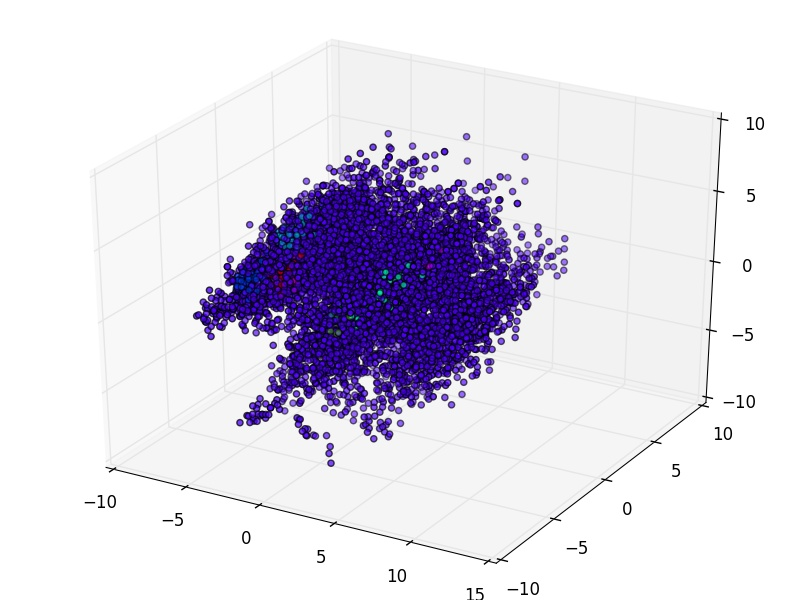
\includegraphics[width=0.5\textwidth]{../img/clusters_occ100_cos.jpg}
    $\mathbb{R}^{101}$: $\spadesuit\clubsuit\blacksquare$
    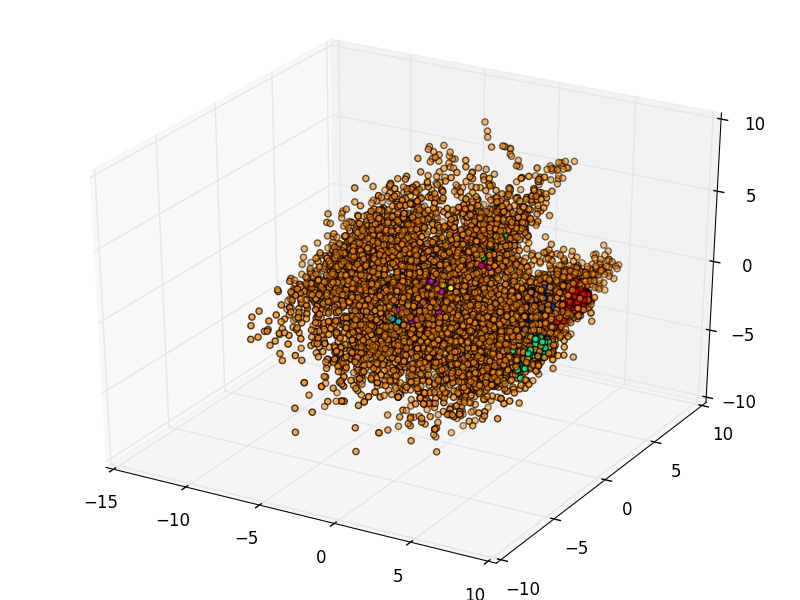
\includegraphics[width=0.5\textwidth]{../img/clusters_occ100_eucl.jpg}
    $\mathbb{R}^{101}$: $\spadesuit\clubsuit\varheart$

    \columnbreak

    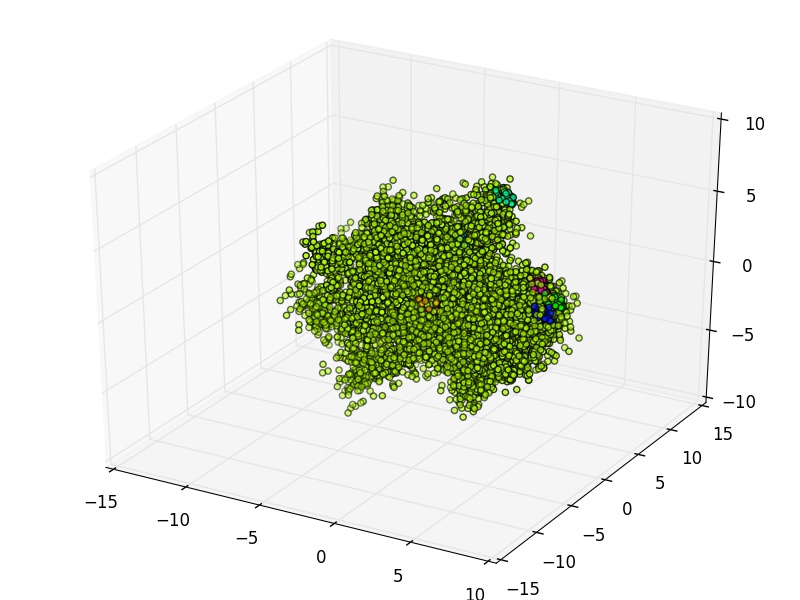
\includegraphics[width=0.5\textwidth]{../img/clusters_occ1.jpg}
    $\mathbb{R}^{100}$: $\spadesuit\bigstar$
    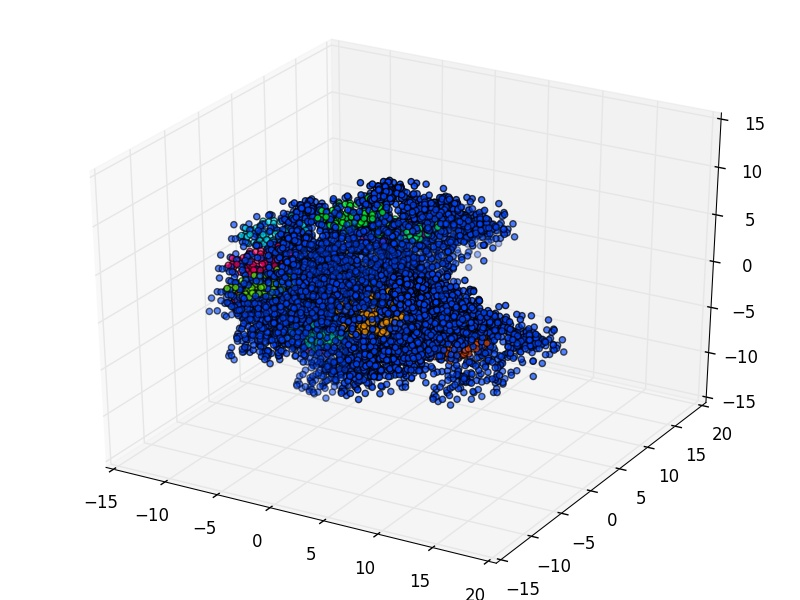
\includegraphics[width=0.5\textwidth]{../img/clusters_occ100_dist_eucl_cos_concat.jpg}
    $\mathbb{R}^{302}$: $\spadesuit\clubsuit\varheart\blacksquare\diamondsuit$
  \end{multicols}

  \flushleft
  \fbox{
  \parbox{\textwidth}{
  \textbf{Feature-Legende}
  \begin{multicols}{2}
  \begin{itemize}
    \item[$\spadesuit$] $\vec{v}(t_2) - \vec{v}(t_1)$
    \item[$\bigstar$] $\Lambda(t_1, t_2) \geq 1$
    \item[$\clubsuit$] $\Lambda(t_1, t_2) \geq 100$
  \end{itemize}
  \columnbreak
  \begin{itemize}
    \item[$\blacksquare$] $cos(\vec{v}(t_2), \vec{v}(t_1))$
    \item[$\varheart$] $\parallel \vec{v}(t_2) - \vec{v}(t_1) \parallel$
    \item[$\diamondsuit$] $\vec{v}(t_2) \oplus \vec{v}(t_1)$
  \end{itemize}
\end{multicols}
}}
  \caption[Dreidimensionale Projektionen einiger durch das Mappingverfahren resultierender Vektorräume]{Dreidimensionale
   Projektionen einiger zufällig ausgewählter, durch das Mappingverfahren resultierender Vektorräume.
   Jeweils dargestellt: 10000 Vektoren. Symbole zeigen die jeweils genutzten Features an, die zu den resultierenden
   Vektoren konkateniert oder im Falle von $\Lambda(\cdot)$ im Vornherein als Filter verwendet werden. Farben
   der Datenpunkte entsprechen der Zugehörigkeit zu einem Cluster.\label{fig:proj_map}}
\end{figure}

\end{itemize}

\subsubsection{Ansatz}

Das Fehlschlagen des Vorgehens kann auch auf einer theoretischen Ebene festgestellt werden: Das Ziel bestand darin, Wissen
über Relationen zwischen Wortpaaren zu extrahieren. Um dieses Wissen gewissermaßen ``freizulegen'', muss es aber auf eine
Art und Weise innerhalb der Daten ``kodiert'' sein, wenn auch implizit (so wie die semantische Ähnlichkeit zwischen Wörtern
durch die räumliche Nähe ihrer Vektoren und deren Dimension kodiert ist).\\
Wie beim Trugschluss am Ende von \ref{sec:zwi-dis-data} gezeigt wurde, sind semantische Relationen nicht eindeutig
innerhalb der Daten festzustelen - bzw. nur dann, wenn bereits vorher bruchstückhaftes Wissen darüber vorliegt. Ohne
dieses Vorwissen sind richtige von nur scheinbaren Relationen nicht zu trennen. Um den Ansatz zukünftig zu einen erfolgreichen
Ende zu führen, müsste also überlegt werden, ihn von einem unüberwachten in einen mindestens semi-überwachten Ansatz zu
transformieren und weiteres Wissen aus einer anderen Domäne hinzuzufügen.
